\documentclass[tikz,border=1mm,10pt]{standalone}
%\usepackage[dvipsnames]{xcolor}
\usepackage{pgfplots}
\pgfplotsset{compat=1.5.1}
\begin{document}
	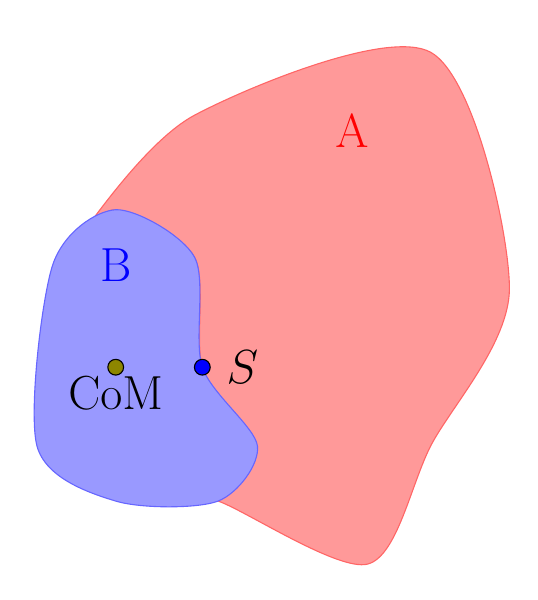
\begin{tikzpicture}
	\draw [color=red!60, fill=red!40] plot [mark=none, smooth  cycle] coordinates {(-0.5,1.6) (0,2) (1,1.4) (1.1,0) (1.7,-1)  (0.8,-1.7) (1.3,-1.7) (3.2, -2.5) (4, -1) (5,1) (4,4)  (1,3.2)};
	\draw [color=blue!60, fill=blue!40] plot [mark=none, smooth  cycle] coordinates {(0,2) (1,1.4) (1.1,0) (1.8,-1) (1.3,-1.7) (0,-1.7) (-1,-1) (-0.8,1.3)};
	
	
	
	\draw [fill=olive] (0,0) circle(.1) node[below] {\LARGE CoM};
	\draw [fill=blue] (1.1,0) circle(.1) node[right] {\LARGE \ $S$};
	\node [red] at (3,3) {\LARGE A};
	\node [blue] at (0,1.3) {\LARGE B};
%	\draw [step=1] (-5,-5) grid (6,6) ;
%	\draw [step=5, very thick] (-5,-5) grid (5,5) ;
	\end{tikzpicture}
\end{document}